\section{Estruturas}

\textbf{Sistema de Armazenamento}
\qquad Segundo orientação dos professores avaliadores no primeiro ponto de controle, o armazenador \label{fig:Estrutura_Visao_Geral} acabou sendo construído em escala, com capacidade de suporte de 50 kg, a fim de diminuir custos e facilitar seu transporte, mesmo embora a estrutura de sustentação e a flutuadora tenham sido construídas em tamanho real. O peso, a diminuição do centro de gravidade e a manutenção da composição química da ração são fatores que contribuíram para a seleção do material do armazenador. Dessa forma, o alumínio foi a opção mais viável a ser escolhida.

\textbf{Sistema de Alimentação}

\qquad O transporte da ração entre o armazenador e o dosador é feito por uma  rosca \label{fig:Rosca1}  e, portanto, o material utilizado foi aço inox, pois não há reatividade entre o material e a ração, além proporcionar uma maior resistência à estrutura. O tubo que envolve a rosca é feito de PVC, tanto pela facilidade de construção, quanto à acessibilidade e durabilidade inerentes ao material diante as condições de uso impostas. \\ \qquad As dimensões do sistema foram aumentadas para se adequar à vazão necessária para que a ração seja despejada no intervalo de tempo correto. Diante disso, além das dimensões da rosca terem sido aumentadas, o dosador também teve que ser redimensionado de 5 kg para 10 kg devido à dinâmica de alimentação dos próprios peixes. Dessa forma, a angulação de escoamento da ração também teve de ser revista.


\textbf{Sistema de Sustentação}

\qquad A estrutura de sustentação \label{fig:Estrutura_Visao_Geral} do alimentador foi confeccionada com cantoneiras de alumínio devido à sua capacidade de sustentar o armazenador, a rosca transportadora, o dosador e os componentes eletrônicos. Além da capacidade de sustentação, o alumínio foi escolhido por evitar a elevação do centro de gravidade em relação ao centro de empuxo. \\ \qquad A estrutura de sustentação flutuadora foi projetada para suportar uma carga de 400 kg de ração e  mais uma massa considerada fixa de 125 kg. Esta última suporta os componentes em tempo integral e, eventualmente, a massa de um ser humano de 100 kg e um saco de ração de 25kg. Dessa forma, foi calculada a estabilidade descrita no PC1 e, então, foi obtida a estabilidade elevada durante toda a transição durante o armazenamento a cheio e a vazio. A escolha do material foi baseada na disponibilidade de mercado e o aumento da massa da estrutura sustentadora que resulta em uma maior estabilidade. Caso o material utilizado fosse o alumínio, assim como no restante de toda a estrutura, complicações como o aumento de custo, perda de estabilidade e complexidade na construção, esta devido ao tipo específico de soldagem, seriam fatores determinantes para a inviabilização da construção do flutuador.


\begin{figure}
\centering
Estrutura Visão Geral
\includegraphics[width=5in]{Estrutura_Visao_Geral}
\linebreak
\end{figure}

\begin{figure}
\centering
Tensões Armazenador
\includegraphics[width=5in]{Armazenador_Tensao}
\linebreak
\end{figure}

\begin{figure}
\centering
Tensões Dosador
\includegraphics[width=5in]{Dosador_Tensao}
\linebreak
\end{figure}

\begin{figure}
\centering
Tensões Estrutura Sustentação
\includegraphics[width=5in]{Sustentacao_Tensao}
\linebreak
\end{figure}

\begin{figure}
\centering
Altura Submersa Máxima
\includegraphics[width=5in]{Altura_max}
\linebreak
\end{figure}

\begin{figure}
\centering
Altura Submersa Mínima
\includegraphics[width=5in]{Altura_min}
\linebreak
\end{figure}

\begin{figure}
\centering
Fator de Segurança Estrutura Sustentação Flutuadora
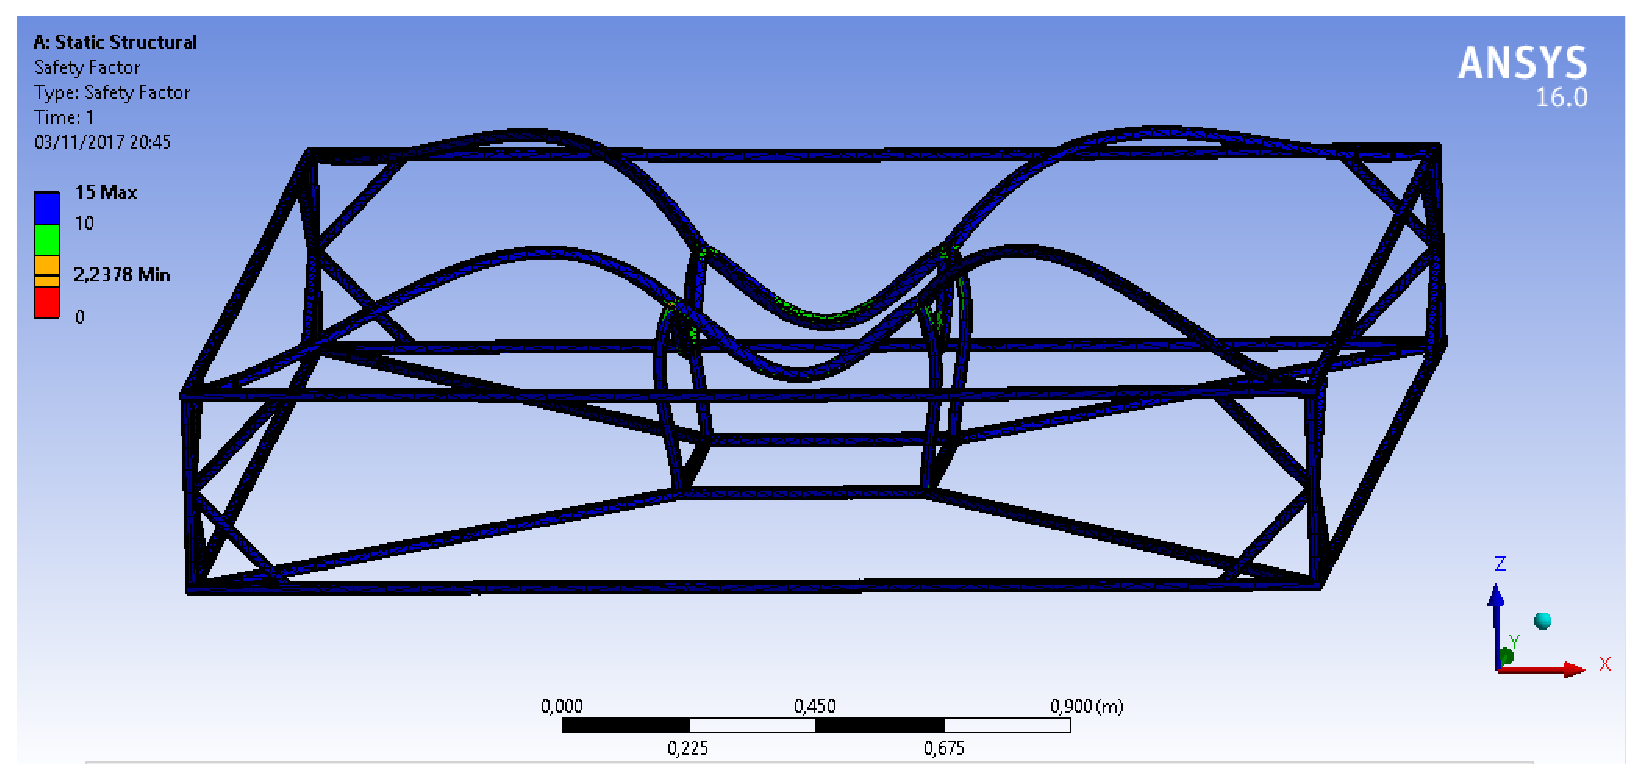
\includegraphics[width=5in]{EstruturaSustentacao_SimulacaoAnsys_FatordeSeguranca}
\linebreak
\end{figure}

\begin{figure}
\centering
Deformação Estrutura Sustentação Flutuadora
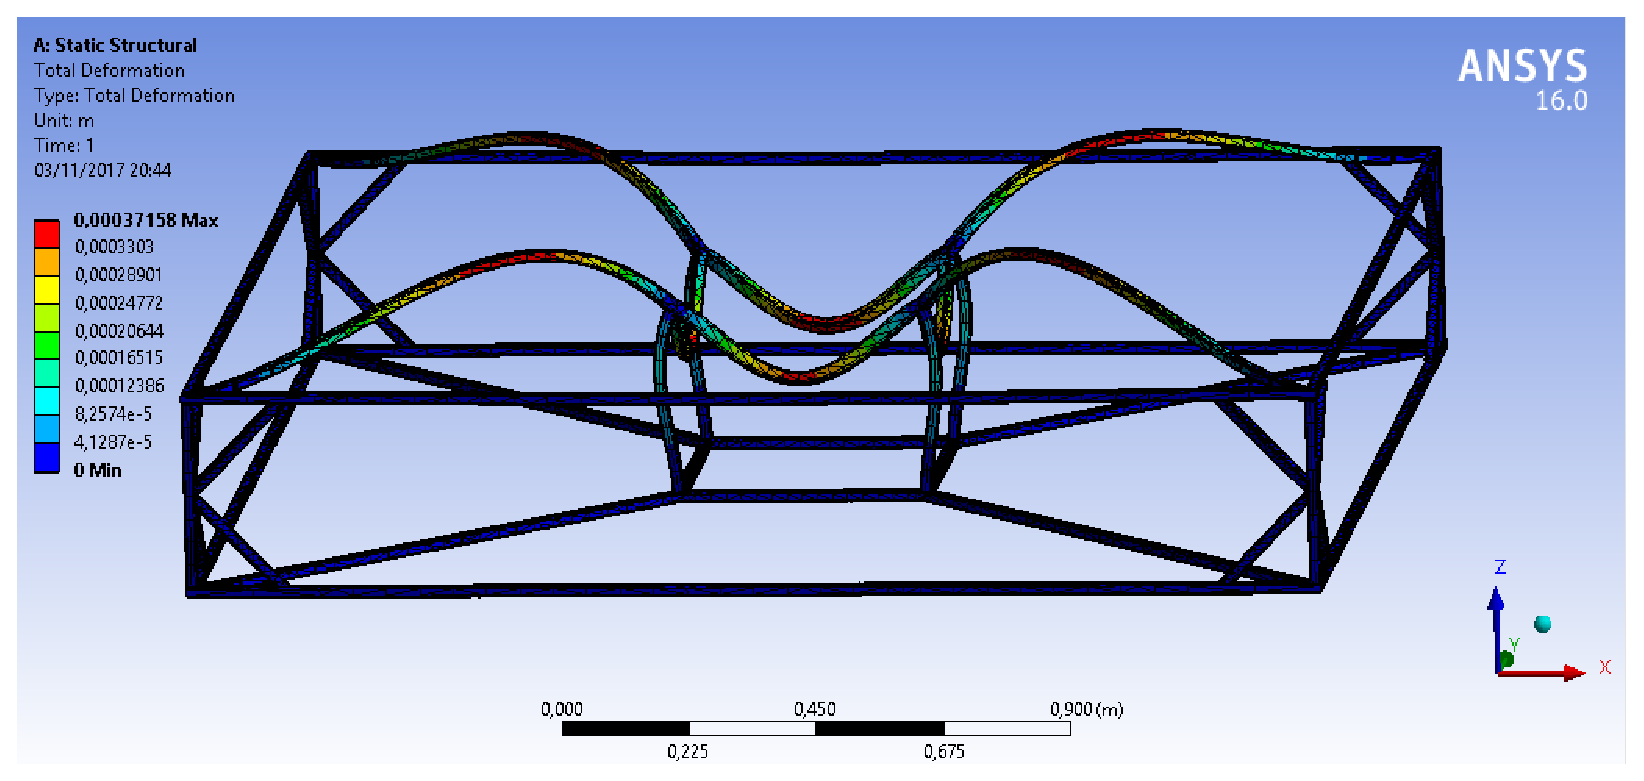
\includegraphics[width=5in]{Deformacao_EstruturaSust}
\linebreak
\end{figure}

\begin{figure}
\centering
Tabela Estabilidade / Altura Submersa / Sobremersa
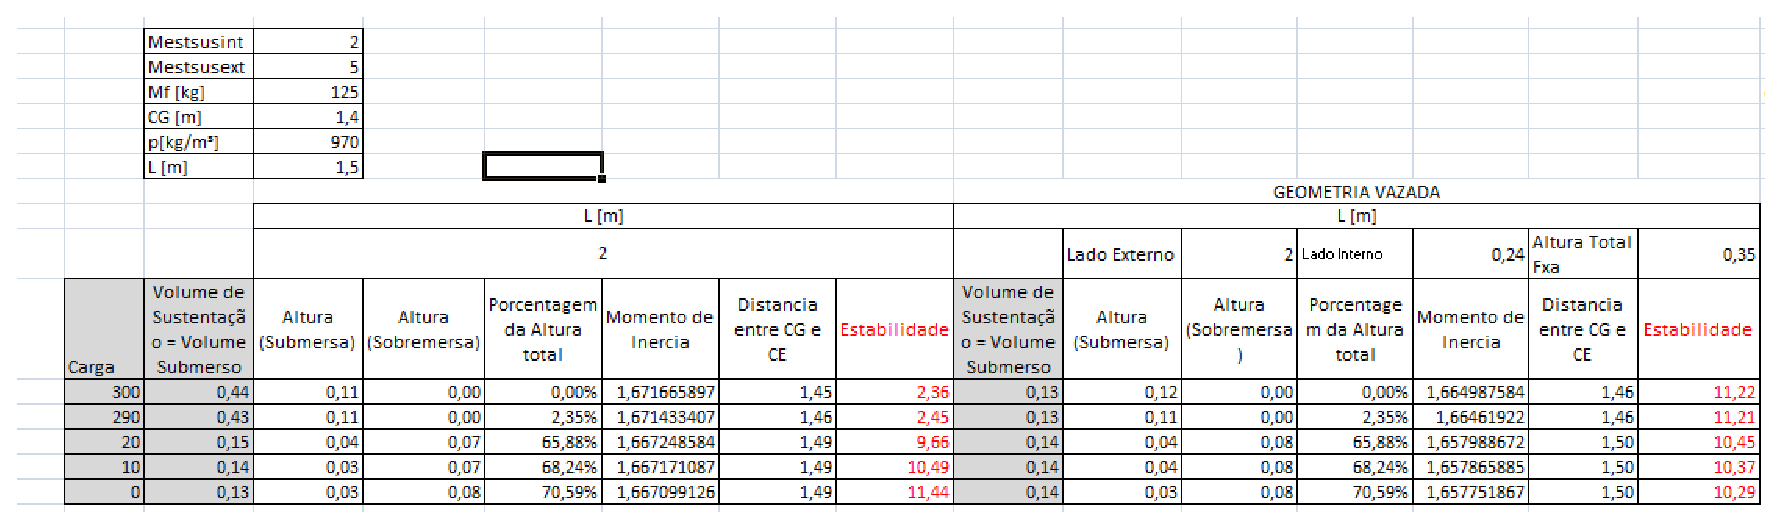
\includegraphics[width=5in]{Tabela_Sustentacao}
\linebreak
\end{figure}

\begin{figure}
\centering
Comparativo Dimensões Estrutura Sustentadora
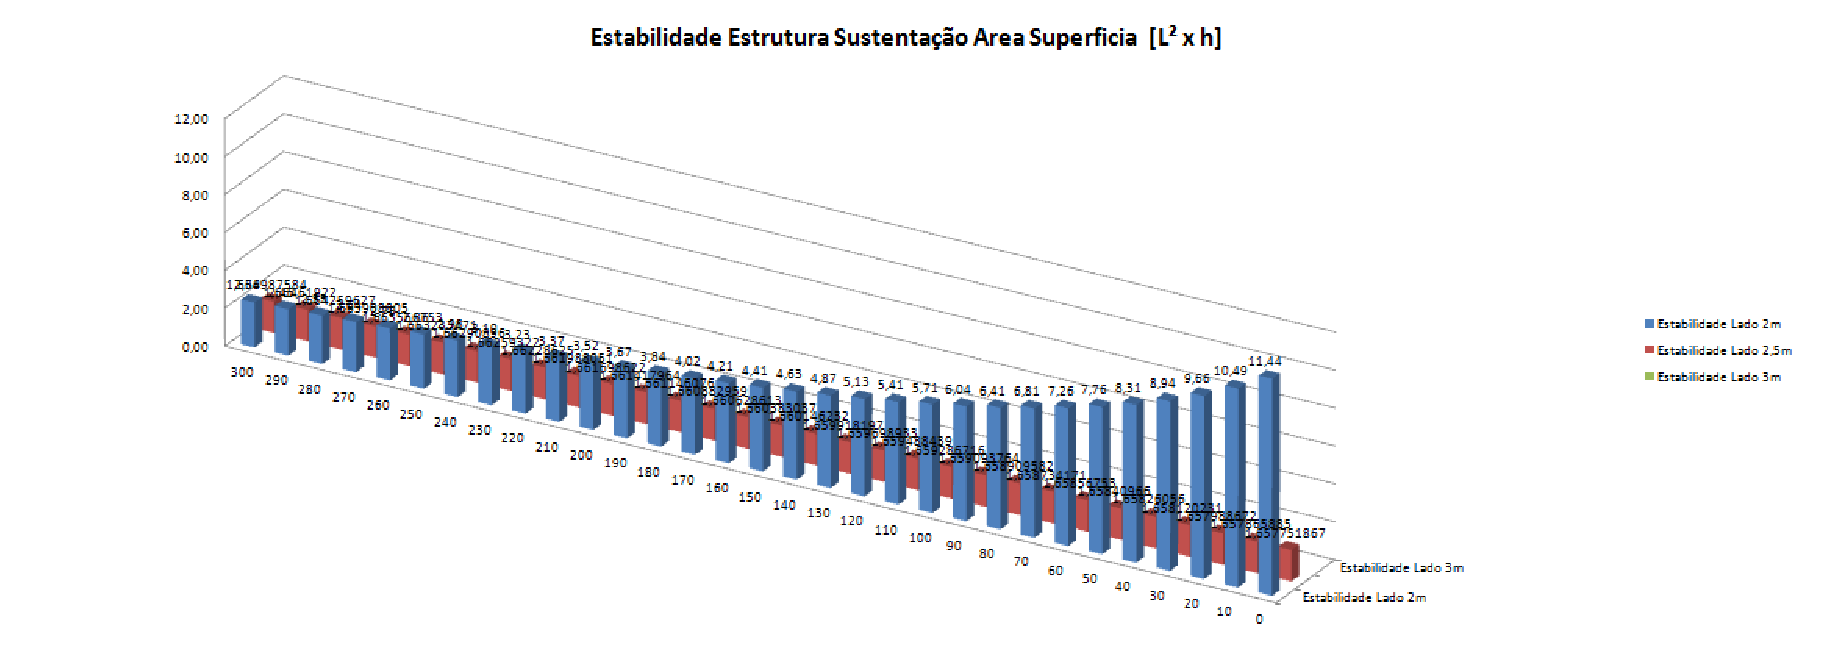
\includegraphics[width=5in]{ComparacaoEstabilidade_EstruturaSustentadora}
\linebreak
\end{figure}

\begin{figure}
\centering
Estrutura
\includegraphics[width=5in]{Estrutura1}
\linebreak
\end{figure}

\begin{figure}
\centering
Estrutura
\includegraphics[width=5in]{Estrutura2}
\linebreak
\end{figure}

\begin{figure}
\centering
Tremonha
\includegraphics[width=5in]{Tremonha1}
\linebreak
\end{figure}

\begin{figure}
\centering
Tremonha
\includegraphics[width=5in]{Tremonha2}
\linebreak
\end{figure}

\begin{figure}
\centering
Tremonha
\includegraphics[width=5in]{Tremonha3}
\linebreak
\end{figure}

\begin{figure}
\centering
Rosca
\includegraphics[width=5in]{Rosca1}
\linebreak
\end{figure}

\begin{figure}
\centering
Rosca
\includegraphics[width=5in]{Rosca2}
\linebreak
\end{figure}



\begin{figure}
\centering
Estrutura Sustentação Flutuadora
\includegraphics[width=5in]{Flutuacao}
\linebreak
\end{figure}

\begin{figure}
\centering
Desenho Mecânico - Aresta Fixação
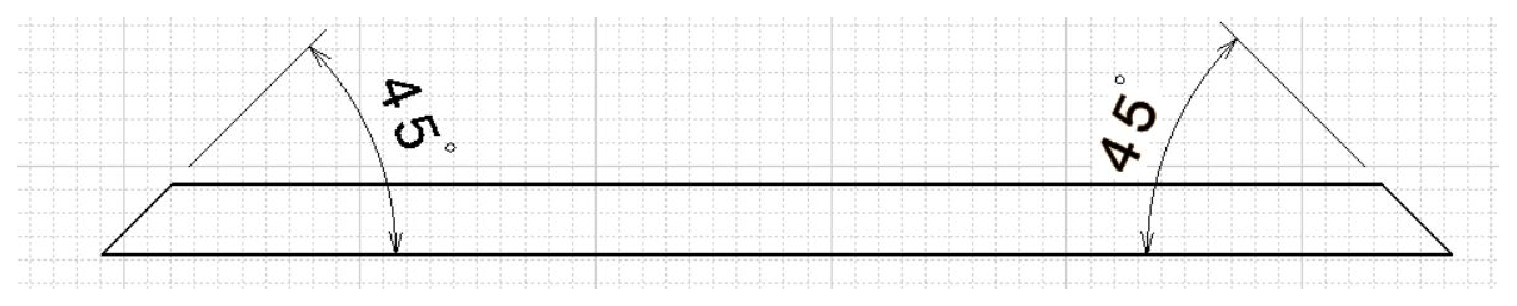
\includegraphics[width=5in]{Aresta_Fixacao}
\linebreak
\end{figure}

\begin{figure}
\centering
Desenho Mecânico - Armazenador Base
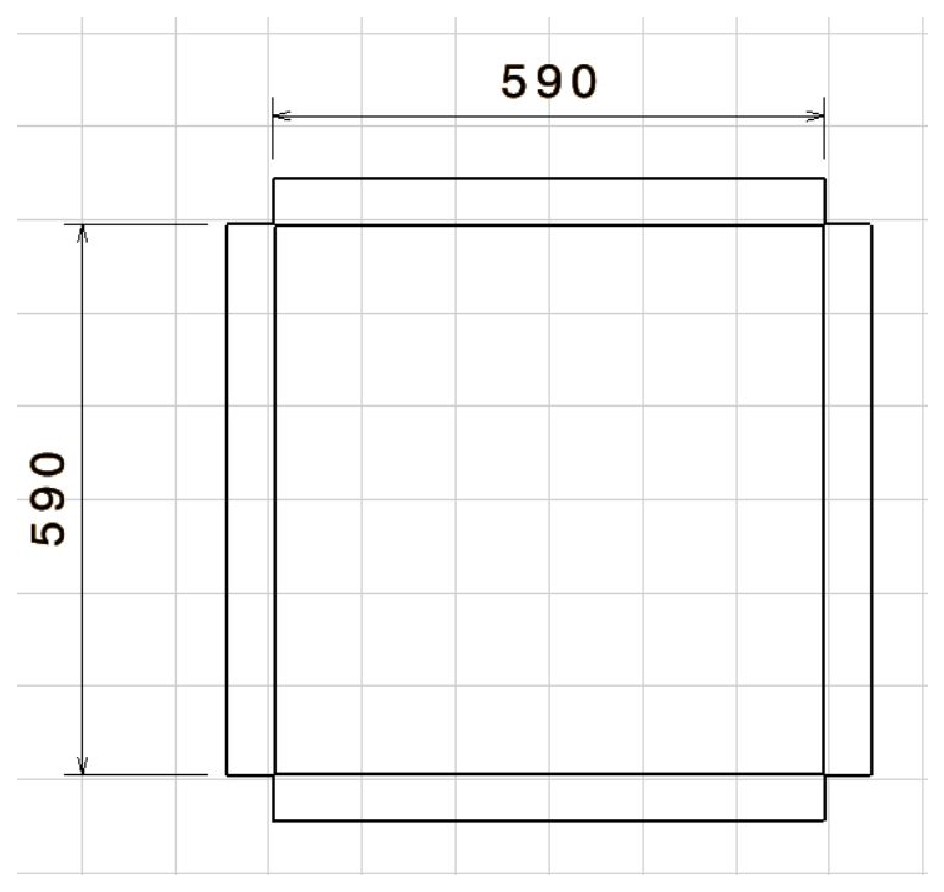
\includegraphics[width=5in]{Armazenador_Base}
\linebreak
\end{figure}

\begin{figure}
\centering
Desenho Mecânico - Armazenador Tremonha
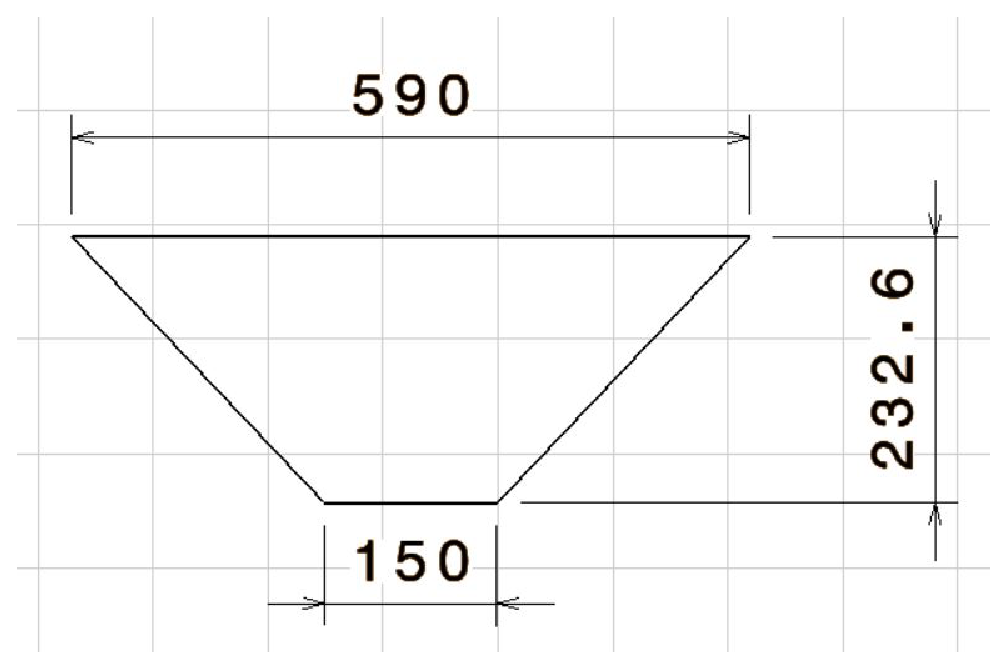
\includegraphics[width=5in]{Armazenador_Tremonha}
\linebreak
\end{figure}

\begin{figure}
\centering
Desenho Mecânico - Case Eletrônicos
\includegraphics[width=5in]{Case_Eletronicos}
\linebreak
\end{figure}

\begin{figure}
\centering
Desenho Mecânico - Dosador Chapas
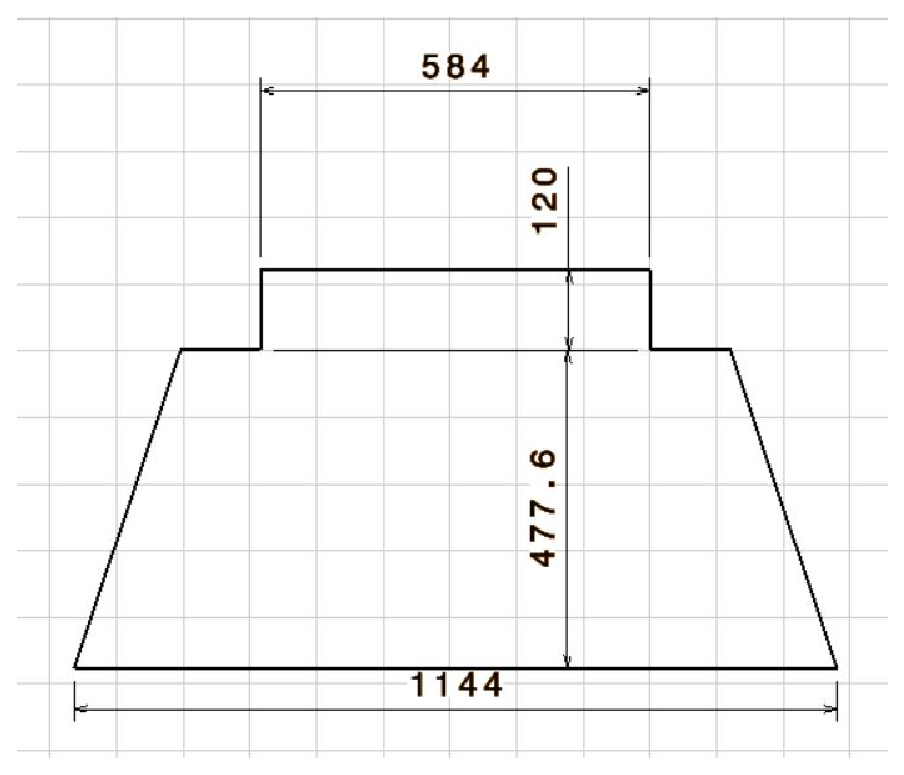
\includegraphics[width=5in]{Dosador_Chapas}
\linebreak
\end{figure}

\begin{figure}
\centering
Desenho Mecânico - Dosador Frente
\includegraphics[width=5in]{Dosador_Frente}
\linebreak
\end{figure}

\begin{figure}
\centering
Desenho Mecânico - Suporte Barra - Dosador
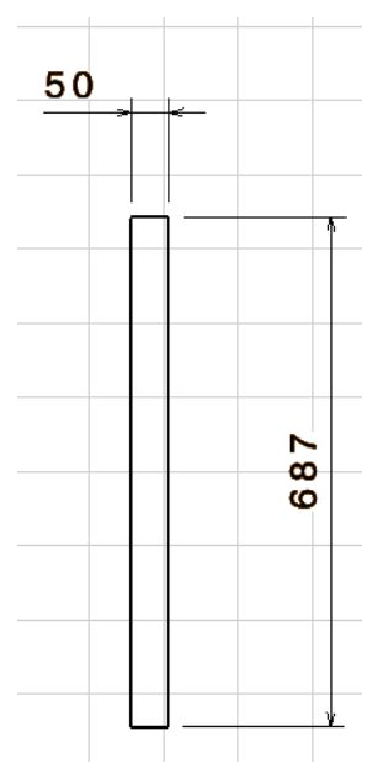
\includegraphics[width=5in]{Suporte_Barra_Dosador}
\linebreak
\end{figure}

\begin{figure}
\centering
Desenho Mecânico - Suporte Colunas
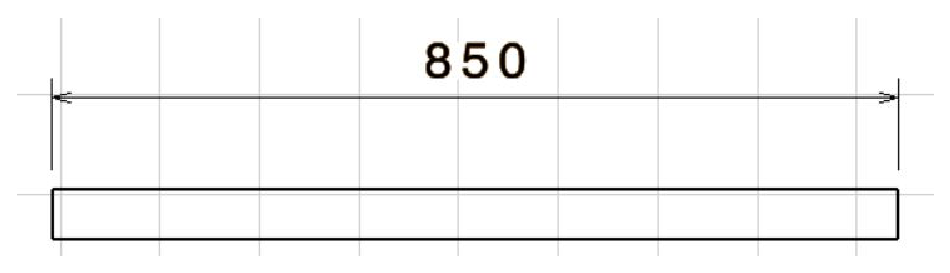
\includegraphics[width=5in]{Suporte_Colunas}
\linebreak
\end{figure}

\begin{figure}
\centering
Desenho Mecânico - Suporte Topo
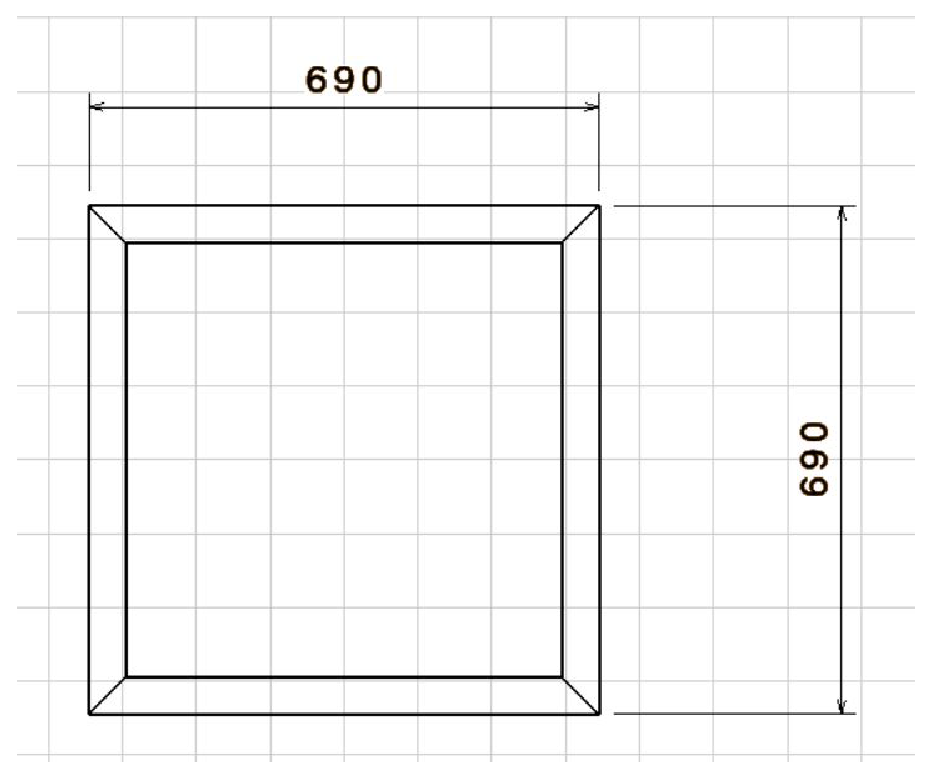
\includegraphics[width=5in]{Suporte_Topo}
\linebreak
\end{figure}
